\section{Théorie}

\begin{minipage}{\textwidth}
    \begin{wrapfigure}{R}{0.5\textwidth}
        \centering
        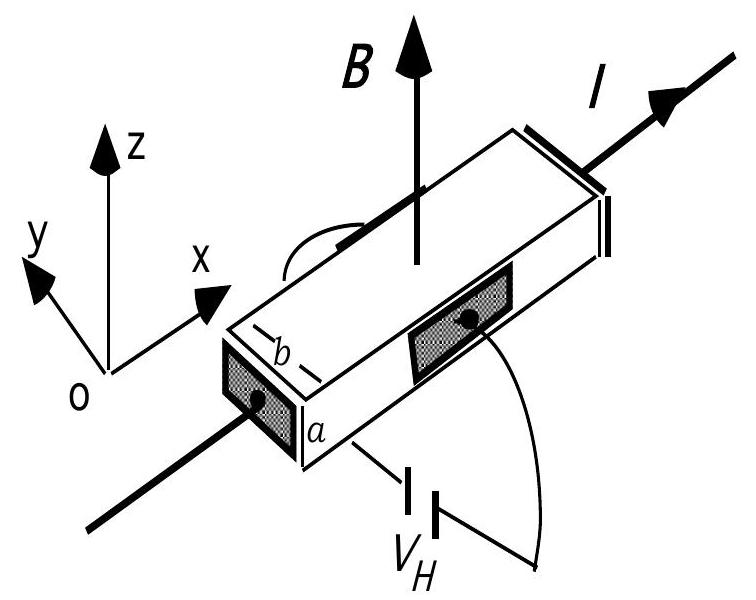
\includegraphics[width=\linewidth]{figures/hall.png}
        \caption{Conducteur électrique de section \(S = a \cdot b\) placé dans un champ magnétique \(\vec{B}\) \cite{notice}}
        \label{fig:hall}
        \vspace*{1cm}
    \end{wrapfigure}

    Lorsqu'un conducteur ou un semiconducteur traversé par un courant est placé dans un champ magnétique, les charges contenues dans ce matériau se déplacent selon une direction perpendiculaire au champ magnétique. Soit le repère carthésien \((\vec{e}_x,\vec{e}_y,\vec{e}_z)\) de la \autoref{fig:hall}. Avec le champ magnétique \(\vec{B}\) orienté selon \(\vec{e}_z\) et le déplacement de charges selon \(\vec{e}_x\), la force de Lorentz \(\vec{F}_L = q\vec{v} \times \vec{B}\) permet d'obtenir que le champ électrique \(\vec{E}\), dû à l'accumulation de charges d'un côté de l'échantillon, est selon \(\vec{e}_y\). La différence de potentiel créée est donc selon cette direction et correspond à la tension de Hall \(V_H\):

    \begin{equation}
        V_H = -E_yb
    \end{equation}

    avec b la largeur de l'échantillon. L'effet Hall, proportionel au champ magnétique et au courant, est donné par l'équation

    \begin{equation}
        V_H = -R_H j_x B_z b
        \label{eq:effet_hall}
    \end{equation}

    avec \(R_H\) la constante de Hall de l'échantillon en [\si{\meter\cubed\per\coulomb}], \(j_x\) la densité de courant traversant l'échantillon selon l'axe \(\vec{e}_x\) et \(B_z\) le champ magnétique selon \(\vec{e}_z\). \cite{notice}
\end{minipage}

Il est possible de montrer à l'aide de l'effet Hall et de la force de Lorentz que la constante de Hall \(R_H\) vaut

\begin{equation}
    R_H = \frac{1}{Nq}
    \label{eq:N}
\end{equation}

avec \(N\) la densité de porteurs de charge en [\si{\per\meter\cubed}] et \(q\) la charge du porteur de charge. Le signe de \(R_H\) permet donc de déterminer le signe des porteurs de charge.\\
En notant que la densité de charge est donnée par \(j = \frac{I}{S}\) où \(I\) est le courant et \(S\) la section de l'échantillon, l'\autoref{eq:effet_hall} donne:

\begin{equation}
    V_H = -R_H \frac{IB}{a} \iff R_H = -\frac{-V_H a}{IB}
    \label{eq:R_H}
\end{equation}

avec \(a\) l'épaisseur de l'echantillon comme indiqué à la \autoref{fig:hall}.
